\documentclass[12pt, letterpaper]{article}  % standard LaTeX, 12 point type
\usepackage{amsfonts,latexsym}
\usepackage{amsthm, amssymb, amsmath}
\usepackage{fancyhdr} %Header package
\usepackage{lastpage}
\usepackage{graphicx}
\usepackage[margin=1in, dvips]{geometry} %1 inch margins.  Get rid of this line
                                         %if you prefer LaTex default formatting
\usepackage{hyperref} %Navigation in TOC and URLs in References
\usepackage{setspace}
\usepackage{float}
\usepackage[export]{adjustbox}
\usepackage{appendix}
\usepackage{mcode}
\usepackage{upquote}
%\input{psfig.sty} % for imported eps files
\pagestyle{fancy}

%%% This LaTeX template is based on the Outstanding SIAM Award winning paper by the MIT team of Spann, Gulotta, and Kane in 2007. 
%%% Template by Andrew Spann, spann @(at) alum .(dot) mit .(dot) edu


% IMPORTANT: Set your team number in the header section after the summary



%%%%%%%%%%%%%%%%%%%%%%%%%%%%%%%%%%%%
%%%%%%%%%%%%%%%%%%%%%%%%%%%%%%%%%%%%
%%%%%%%%%%%%%%%%%%%%%%%%%%%%%%%%%%%%

%%%Preamble
%%  You can skip this part if you are not doing anything complicated


% This gets rid of LaTeX's tendency to wrap lines over-
% zealously.  The numbers are arbitrary.  Set it to over 9000 if you wish.
\hyphenpenalty=8000 \tolerance=1000


% Here are some suggested custom commands that you may find useful.  You can comment these out if you don't want them.  Most of these were suggested by MIT Professor Richard Stanley in his 18.091 mathematical exposition class.
\newtheorem{theorem}{Theorem}[section]
\newtheorem{proposition}[theorem]{Proposition}
\newtheorem{lemma}[theorem]{Lemma}
\newtheorem{corollary}[theorem]{Corollary}
\newtheorem{conjecture}[theorem]{Conjecture}

\theoremstyle{definition}
\newtheorem{example}{Example}[section]

% unnumbered environments:
\theoremstyle{remark}
\newtheorem*{remark}{Remark}
\newtheorem*{notation}{Notation}
\newtheorem*{note}{Note}

\newtheorem{thm}{Theorem}
\newtheorem{lem}[thm]{Lemma}
\theoremstyle{plain}
\newtheorem*{defn}{Definition}

% Richard Stanley's favorite macros
\newcommand{\CC}{\mathbb C} % blackboard math , for ``complex,'' etc
%\newcommand{\qed}{$\Box$}      % box  indicating end of proof.
% for a sequence of unnumbered displayed equations:
\newcommand{\beas}{\begin{eqnarray*}}
\newcommand{\eeas}{\end{eqnarray*}}
\newcommand{\bm}[1]{{\mbox{\boldmath $#1$}}} % for boldface math symbols


% More examples of LaTex macros, actually used in 2007 paper.
%\newcommand{\E}[1]{\textrm{E}\left[#1\right]}
%\newcommand{\V}[1]{\textrm{Var}\left[#1\right]}
%\newcommand{\SizeError}{2\%}
%\newcommand{\Cov}[2]{\textrm{Cov}\left(#1,#2 \right)}



% Blank parts of the header.  The rest is updated after the summary.
\lhead{ } \chead{ } \rhead{ } \cfoot{ }

%%%%%%%%%%%%%%%%%%%%%%%%%%%%%%%%%%%%%%%%%%%%
%%%%%%%%%%%%%%%%%%%%%%%%%%%%%%%%%%%%%%%%%%%%

\begin{document}

\ \vspace{0.3in} %%%%%%%%%%%%%  Summary  %%%%%%%%%%%%%%%%%%%%%%%%%%%%%

\begin{center}
\Large  %Your title here    \\
%Second line/subtitle if needed
\end{center}

\ \normalsize \\
%%% Type your summary here.  The summary is important, so leave enough time at the end to write it.  Remember to focus on your methodology and results in the summary, don't waste too much time on introduction material.  My 2007 summary is listed below in comments for your reference.



We build from the ground up a computer simulation of a search of missing aircraft.  We populate a rectangular search domain with a grid of cells of location density and define an “enjoyment function” where visitors gain points for going on rides and lose points as they stand in line.  We propose two QuickPass systems.  In the Appointment System, QuickPasses represent an appointment to visit the ride later that day.  In the Placeholder System, a QuickPass represents a virtual place in line.  We then choose test cases to represent both systems and run the computer simulation.  With each set of parameters, we adjust the probability weights that govern visitor behavior to fit a Nash Equilibrium.  The Nash equilibrium adapts the behavior of park visitors to a greedy equilibrium that is not optimal for the group, but is representative of human individuals giving weight to decisions based on what is correlated with giving them an immediate benefit.  
Our results suggest that it is in the park’s best interest to allocate a high percentage of the rides to QuickPass.  Reserving too few seats on a ride for QuickPass users can result in average visitor enjoyment being lower than if there were no QuickPass system at all.  Both the Placeholder System and the variant of the Appointment System with 75% of ride capacity allocated to QuickPass users show strong increases in visitor enjoyment.  Varying the length of the time window that the QuickPass is valid for has little effect on visitor enjoyment.  








%%%%Spann, Gulotta, Kane 2007 summary for the Congressional Redistricting (gerrymandering) problem:

%We propose and evaluate two methods for determining congressional
%districts. The models are defined so that they only explicitly
%contain criteria for population equality and compactness, but we
%show through a detailed analysis that other fairness criteria such
%as contiguity and city integrity are present as emergent properties.

%In the Moment of Inertia Method, districts are created such that
%populations are within $\SizeError$ of the mean district size and
%the sum of the squares of distances between each census tract
%weighted by population size and the district's centroid is
%minimized.  We present a mathematical argument that this model will
%result in districts that are convex.

%In the Diminishing Halves Method, the state is recursively divided
%in half by a line that is perpendicular to the statistical best-fit
%line describing the region's census tracts.

We are able to parse past 50 years of aircraft accident
data, extracting the root cause of the accidents and their typical response (glide, free fall etc.). By parsing these data, we are able to construct distributions of probable crash radius with a relatively high confidence.  We run our algorithms on three different types of aircrafts, G280 (small), B737-900ER (medium), and Airbus 380 (large).

%We compare the results of our methods to each other and to the
%current districts in the respective states.  Both our algorithms
%return districts that are not only contiguous but also convex, aside
%from borders where the state itself is nonconvex.  We superimpose
%city locations on the district maps to check for community
%integrity. We evaluate our proposed districts with the Inverse Roeck
%Test, the Length-Width Test, and the Schwartzberg Test to obtain
%quantitative measures of compactness.

%The initial conditions do not greatly affect the Moment of Inertia
%Method.  We run additional variants of the Diminishing Halves Method
%and find that they do not improve over our normal method.
%\medskip

%Based on our results, we would like to recommend to states that
%\begin{itemize}
%\item District shapes should be convex.
%\item City boundaries and contiguity can be emergent properties, not explicit considerations.
%\item A good algorithm can handle states of different sizes.
%\item We recommend our Moment of Inertia Method, as it
%consistently performed the best.
%\end{itemize}



\newpage

%%%%%%%%%%%%%%%%%%%%%%%%%%%%%%%%%%%%%%%%%%%%%%

% IMPORTANT  !!!!!
% IMPORTANT  !!!!!
% SET YOUR TEAM NUMBER BELOW:

\lhead{Team 41747}  \rhead{Table of Contents} \doublespacing

%I'm using doublespacing.  If you don't want that, get rid of the tag above.

%Using LaTeX gives you a table of contents for free!
\tableofcontents
\ \\

\newpage

% Having completed the summary, now we define the header
\setcounter{page}{1} \chead{Section \thesection}  \rhead{Page
\thepage\ of \pageref{LastPage}}



%%%%%%%%%%%%%%%%%%%%%%%%%%%%%%%%%%%%%%%%%%%%%%%%%%%%%%%%%%%%%%%%

\section{Problem Restatement}\label{sec:restate}
%% One quick paragraph describing the problem and foreshadowing your approach.

Concerns over the disappearance of flight MH370 have rekindled interests on how to devise an optimal search plan to maximize our chance at finding the debris of an aircraft lost in a vast open body of water. Given the last known state of the aircraft, we wish to construct a probability distribution of the aircraft debris to and then a search plan that can assist the search-and-rescue teams in allocation of their efforts. Since we fear that the plane have been crashed, we assume no signals can be received from the lost plane, and we ignore the possibility that no foul-play or navigation error could be the only cause for lost of contact with the aircraft.

The specific factors that should be taken into account in obtaining such optimal search plan
include the variation in the type of crashed airplane and that of the search agents. Furthermore, we must first determine what constitutes the optimality of a search plan. Once the objective function is determined, the planning problem now turns into one of the optimization and we must
determine an efficient and robust way to compute the search plan.


%%%%%%%%%%%%%%%%%%%%%%%%%%%%%%%%%%%%%%%%%%%%%%%%%%%%%%%%%%%%%%%%%%%%
%%% Uncomment if needed
\section{Acronyms and Terms}\label{sec:terms}

\begin{itemize}
\item \textbf{SAR}. Search-And-Rescue.

\item \textbf{MTOW}. Maximum Take Off Weight.

\item \textbf{USCG}. United States Coast Guards.
\item \textbf{SAROPS}. Search and Rescue Optimal Planning System.
\item \textbf{IMTS}. Informational Moving Target Search.

\item \textbf{Location Density}. Informational Moving Target Search.
\item \textbf{Search Density}. Informational Moving Target Search.
\item \textbf{Search Effort}. Informational Moving Target Search.
\item \textbf{(Detector) Range Law}. Informational Moving Target Search.
%and so on

\end{itemize}

%%%%%%%%%%%%%%%%%%%%%%%%%%%%%%%%%%%%%%%%%%%%%%%%%%%%%%%%%%%%%%%%%%%%

\section{Assumptions and their Justifications}\label{sec:assumptions}

\textit{\textbf{About the Search Domain and the Missing Aircraft}}
\begin{itemize}
\item \textbf{The search domain $\Omega$ is a $500$km by $300$km rectangle of unobstructed ocean.} This rectangle would cover the whole uncertainty range based on 
the last known state of the lost aircraft for an interval of 15 minutes to 1 hour based on INMARSAT's "Log-on Interrogation" old and newly recommended standards in light of the MH370 accident\textbf{[citation]}.
\item \textbf{The missing aircraft is assumed to be still in this domain at $t=0$.} Although escaping the domain at a later time is allowed.
\item \textbf{The SAR targets remain clustered.} This means that the targets always stay in the same cell on the discretized grid. This assumption is valid as long as the search is initiated close to the incident time and no serve weather condition causes disturbances.
\item \textbf{There are buoyant indicator of target location at all time.} Since no underwater search is performed, we assume that either our SAR objective (e.g. survivors, life rafts, parts of crashed debris) remain buoyant throughout our search planning, or our sensor can detect signs of the objectives 
\item \textbf{The local trajectory of concern is straight}. In addition to the obvious smoothness arguments, it is always possible to apply a conformal transform on the entire search domain to obtain a solution based on a curved trajectory.

\item \textbf{The trajectory from incident to crash is in a straight line.} Even in the worse case of gliding due to single engine failure, the average time from initial to of roughly $10$ minutes based on our analysis. And during this time any banking maneuver is unlikely to cause significant deviation of the aircraft location density in terms of our discretized cells.
\item \textbf{Hijacking or on-board navigation system only problems are not the cause of the incident}. This means that we assume the aircraft is crashed and assumes only the dynamics of the ocean and wind in our search domain. Although hijacking incidents account for nearly $20$\% of all accidents in past 50 years \textbf{Citation!}, the search agents in consideration (e.g. low flying aircrafts and surface vessel) are largely useless in finding a rouge cruising plane. Also see Section \ref{sec:restate}.
\item \textbf{The missing aircraft can be accurately modeled as either G280, Boeing 737-900ER, or Airbus 380.} These three types of aircraft are well-known representatives of small private/business jets, medium range commercial flights, and large international flights. Cruise speed and other aircraft form factors (e.g. Lift to Drag ratio) are derived based on this assumption.
\item \textbf{The crash radius of the aircraft is only a function of the cause of the incident and the type of the aircraft.} In addition, we assume that the historical distribution of the cause of the accidents is a reasonable prior for the current incident at hand, and it is it is invariant with respect to the type of the aircraft\footnote{We do not have an aircraft aficionado at hand to sift through and separate the accident records based on size}.
\item \textbf{The crash radius calculations assumes constant air density and constant cruise altitude regarless of the types of aircraft involved.} This is not going to be a significant source of error in comparison to other assumptions.
\item \textbf{Aircraft is operating at MTOW}. Assuming this is why we absolutely need an optimal search plan to find the cargos and passengers ASAP.
%%%Add more items as needed
%%%Add more items as needed
\end{itemize}

\ \\
\textit{\textbf{About Debris Drifting}}
\begin{itemize}
\item \textbf{The local drift direction and speed can be accurately modeled as constant within each cell.} Operationally, the resolution of the cells can be adapted to actual drift data.
\item \textbf{Nothing outside the search domain drifts back into it.} This assumption only makes searching harder so good for us.
\end{itemize}

\ \\
\textit{\textbf{About the Search Agents}}
\begin{itemize}
\item \textbf{All agents are commanded and controlled by the central planner at each update interval.} No command and control overhead is assumed for the sake of simplicity.
\item \textbf{Agents arrive at the boundary of the search domain at $t=0$}.  Search agents are assumed to have arrived on the edge of the search domain at $t=0$.
\item \textbf{Unlimited bandwidth between search agent communications}.  This is necessary from a planning perspective as to ignore the less than pertinent issues with sensor fusion and coordination. Moreover, this factor is more than likely fixed by the hardware.
\item \textbf{Search agents are assumed to be either helicopters, UAVs, and surface vessels, all equipped with a bi-variate Gaussian/ definite range law detection probability function.} Moreover, all types of agents are assumed to h Although the problem only mentions "search planes," Marine SAR vessels are very commonly used.
\item \textbf{Search agents admit a detector range law of a bivariate Gaussian as a function of their type, altitude, and speed.} Most sensors used for marine SAR (e.g. magnetometer or camera) behaves roughly according to this distribution. Furthermore, the exact sensor range law varies greatly\footnote{We were not able to find good data on this subject} and we can always use actual measured data in operations. And finally, the detection statistics also follows Koopman's Random search formula \cite{46koopman}.
\item \textbf{The agents all have null probability of false alarm.} According to \cite{83stone} and \cite{13kagan}, this assumption is a standard one employed by the SAR planning industry. It is an reasonable assumption in that usually false alarms for SAR can be resolved quickly and locally (i.e. reexamining the targets are usually an easy task).
\item \textbf{The search agents have zero knowledge of local ocean/wind drift information.} Although modern planning softwares used by professional SAR entities (e.g. SAROPS by U.S. Coast Guards) all have existing database to accommodate real-time ocean drifting \cite{10uscg}, these data are often not precise, not to mention useless on our fictitious geography.
\item \textbf{Operational range and refueling problems are neglected.} In operation, search agents can request refueling vehicles etc. and the time is not quite relevant.
\item \textbf{Agents move in either the horizontal or vertical direction.} Although this is clearly not so realistic operationally, we can always approximate the real search trajectories better by increasing grid resolution.
\item \textbf{Search agent trajectories are known and executed exactly.} This assumption is alliveated by the fact that we do not assume a definite range law.

%%%Add more items as needed
\end{itemize}


%%Uncomment below if you want to begin the next section on a newpage:
%\newpage

%%%%%%%%%%%%%%%%%%%%%%%%%%%%%%%%%%%%%%%%%%%%%%%%%%%%%%%%%%%%%%%%%%%%

\section{Literature Review}\label{sec:litrev}

%% Maybe this isn't relevant to your paper or you want to just name this section as "INTRODUCTION".  There's a bit of flexibility as to what you can do now, so name this and the next few sections in whatever way fits the flow of your paper.  If convenient, I personally like to give a bit of scholarly journal background in some of my papers, but we don't do that every year depending on how weird the problems are.

The problem of finding the optimal search strategy of a target in a fixed region like a body of water, known in the literature as the ``Search and Screening Problem" had been extensively researched and analyzed by generations of researchers of operational research. First aroused as a naval problem, Koopman \cite{46koopman} established the foundation on how to approach this problem. In his seminal papers, many reasonable assumptions as well as useful probability functions and formulas (e.g. the random-search formula) are devised and still in use today.

Stone analyzed the overall development of this field up to 1983 in \cite{83stone}.


In \cite{13kagan}, Kagan and Ben-Gal composed more recent progress on this old problem. The optimal search plan algorithm used later in this paper is derived from their IMTS methods.




%%Uncomment below if you want to begin the next section on a newpage:
%\newpage

%%%%%%%%%%%%%%%%%%%%%%%%%%%%%%%%%%%%%%%%%%%%%%%%%%%%%%%%%%%%%%%%%%%%

\section{Criteria for Optimal Solution}\label{sec:measure}

%% The problem usually doesn't give you a very specific definition for what the ``best'' solution is, so you should clearly explain it.  Feel free to rename this section something more relevant or use a different style and structure for the paper, just make sure you fulfill the goal of defining what the ``best'' solution looks like.

In real life, the only success criterion is whether we can find the target and how long it takes us to do so. However, from the standpoint of search plan optimization, what we want is \textbf{to maximize the likelihood of detection given a fixed search effort}.

%\newpage

%%%%%%%%%%%%%%%%%%%%%%%%%%%%%%%%%%%%%%%%%%%%%%%%%%%%%%%%%%%%%%%%%%%%
\section{Debris Density and Search Planning}\label{sec:mainmethod}
%% (Change the section title of course)

%% Describe your mathematical model and list all relevant equations.  Remember to make your paper easy to skim by placing variable definitions by all equations.  We prefer to use actual words for variables if that variable will only be used once or twice.  Don't use Greek letters unless your variable is directly analogous to what a Greek letter usually means in math or physics.  Feel free to write important sentences \textbf{in bold} to make your paper easier to skim.


Our model uses the probability of each cause of aircraft crash as a premise. This probability comes from our analysis of the data on . For ease of analysis, The causes were then clubbed into four major categories – fire, collision, and engine failure.

First step is to model the probable crash radius of the aircraft in question. To do this, we noted the total number and root cause of commercial aircraft accidents since 1957. From the cruise velocity and cruising altitude of the approximate size of the aircraft as well as the mode of response in reaction to the cause of the accident, we can categorize the data into 4 scenarios: free fall, gliding, impact, and others. (Note: Hijacking and navigation error only incidents were excluded per assumptions. See Section \ref{sec:assumptions}.)

For example, when facing an fire emergency on board, we assume that the airplane would descend in free fall with its initial cruise velocity since it is unlikely that the pilots can initiate significant correction maneuver due to chaos on board.

In

, is considered to be descending in presence of air resistance. For simplicity's sake, the density of air is considered constant and doesn't change with altitude. Furthermore, using the cruise speed of individual aircrafts as the only velocity at the time of the mishap, simple trigonometry along with air resistance calculation leads us to the most probable distance where the debris might have fallen.

Imperfections with our model can always be improved by a more detailed analysis of previous accidents 

\begin{center}
	\begin{figure}[H]
		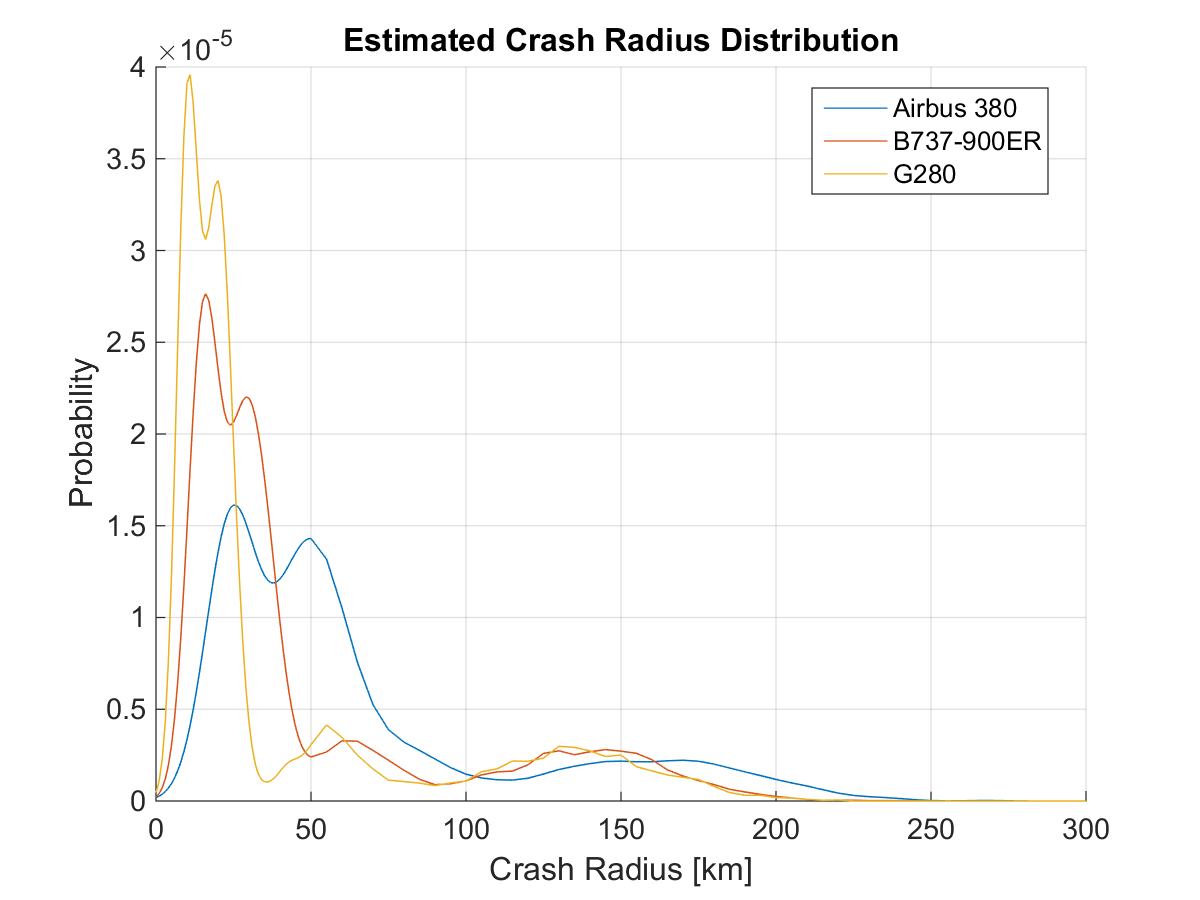
\includegraphics[width=0.9\linewidth]{simulation/CrashRadiusExplain.png}
		\caption{Estimated Crash Radius Distribution of three types of missing aircraft}
		\label{fig:CrashRadius}
	\end{figure}
\end{center}


\subsection{Description}\label{subsecmeth:desc}

%% Maybe you want to split this section into subsections.  Just suggesting things here.  Change as you see fit.  
%% By the way, you don't have to fill out the \label{}'s if you don't want to.  They're so you can \ref{} in the middle of the paper then move entire sections around later without breaking your numbering.


\subsection{Mathematical Interpretation}\label{subsecDist:math}

%% Here's quick lesson on equations if you need it:


\begin{center}
	\begin{figure}[H]
		\centering
		\adjincludegraphics[width=0.5\linewidth,trim={{.3\width} {.45\height} {.3\width} {.2\height}},clip]{simulation/LocationDensityExplain.png}
		\caption{Illustration of the accident geometry. The left {\large $\times$} represents the last known location, the right {\large $\times$} first checkpoint where the aircraft was not found. The incident site is marked by the red {\huge $\ast$}, while the crash site is marked by the black {\huge $\ast$}.}
		\label{fig:CrashRadius}
	\end{figure}
\end{center}

The initial location density at each point away from the intended trajectory is calculated as

\[P[crash\,at\,\text{\huge $\ast$}] = \int P[crash\,radius=\tilde{R}(\tilde{r})]\cdot P[Deviation=\theta(\tilde{R}(\tilde{r}))]\,d\tilde{r}\]

Finally, the probability that the aircraft crashed within one cell is obtained through the double integral.
%\begin{equation}\label{eqn:}
% Type equation as if it were in between $ $ but you don't need the $.
%\end{equation}


%\begin{align*}
%\end{align*}

%%%% Use & to split columns in align mode.  The * is optional, makes the equation not have a number.  You can have as many &'s per line as needed.

Let us recall the definitions and notation which were applied in the search and screening
methods (Section 2.1.1). Assume that the sample space X ={x1,x2,...,xn} represents a
rectangular geographical domain of size (n1,n2), n = n1 × n2, and the points xi ∈ X, i =
1, 2,...,n, represent the cells in which the target can be located at any time t = 0, 1, 2,....
As indicated above, we index the points of X in a linear order such that for the Cartesian
coordinates (j1,j2) of the point xi, its index is given by i = ((j1 − 1)n1 + j2), where
j1 = 1,...,n1 and j2 = 1,...,n2.
The target location probabilities at time t, t = 0, 1, 2,..., are denoted by pt(xi) =
Pr{xt = xi}, i = 1, 2,...,n, where xt ∈ X denotes the target location at time t. As usual,
we assume that 0 ≤ pt(xi) ≤ 1 and
鬀n
i=1 pt(xi) = 1. The target’s movement is governed
by a discrete Markov process with transition probability matrix ρ ==ρij靀n×n, where ρij =
Pr{xt+1 = xj|xt = xi} and 鷀jn=1 ρij = 1 for each i = 1,2,...,n.Ifmatrixρ is a unit
matrix, then the target is static, otherwise we say that it is moving. Given target loca-
tion probabilities pt(x), x ∈ X, at time t, location probabilities at the next time t + 1are
calculated as pt+1(xi) = 鍰jn=1 ρij pt(xi), i = 1, 2,...,n.
The searcher moves over the sample space and at each time t, t = 0, 1, 2,..., looks
for a target by testing a neighboring observed area At ⊂ X of a certain radius r>0, which
is defined by using the metric of the considered geographical domain. Similar to the Singh
and Krishnamurthy model (see Section 3.3.1), we do not restrict the size of the available
observed areas, but assume that the areas have equal size and the trajectory of the searcher
is continuous, as shown in Figure 2.7.



\subsection{Comparison to U.S.C.G. SAROPS}\label{subsec:sarops}

%% Once again, change the sections as you see fit.  

%% Other command suggestions:
%\begin{lem}\label{biglem}
%\end{lem}

%\begin{proof}[Proof of Theorem \ref{algtheorem}]
%\end{proof}

%\section{}\label{labelme}

In comparison to the direct Monte Carlo / particle filter approach employed by the U.S. Coast Guards' SAROPS system, our search planning algorithm
\begin{itemize}
	\item \textbf{do not use multiple senarios.} due to problem statement; More see \ref{sec:assumptions}
	\item \textbf{ss}
\end{itemize}


\subsection{Comparison to SLS Methods}\label{subsec:newer}



%\newpage

%%%%%%%%%%%%%%%%%%%%%%%%%%%%%%%%%%%%%%%%%%%%%%%%%%%%%%%%%%%%%%%%%%
\section{Comparison to a Parallel Search Plan}\label{sec:greedyalg}

%%% Besides your main model, always have a ``control'' algorithm to compare to.  It's even better if you can think of an extra ``good'' algorithm as well.  

Naively, one can also devise the classic parallel search plan where the search agents travel in parallel lines that each agent's observed area overlaps. Such a plan is analyzed in fair amount of detail by Stone in \cite{83stone}. In our crude simulation, we assume that the trajectory of the search agents are known and executed exactly






%\newpage
%%%%%%%%%%%%%%%%%%%%%%%%%%%%%%%%%%%%%%%%%%%%%%%%%%%%%%%%%%%%%%%%%%
%\section{Comparison to a "Steepest Decent" Search Plan}\label{sec:greedyalg}
%
%%%% Besides your main model, always have a ``control'' algorithm to compare to.  It's even better if you can think of an extra ``good'' algorithm as well.  
%
%
%
%also multiple agent/single agent etc.
%
%
%

%\newpage

%%%%%%%%%%%%%%%%%%%%%%%%%%%%%%%%%%%%%%%%%%%%%%%%%%%%%%%%%%%%%%%%%%
\section{Experimental Setup}\label{sec:experiment}
%% State clearly what you are testing.  State your input data and what probability distributions were used in generating it.  Talk a little bit about the implementation of your program (language, if something works a bit differently than the mathematical description you already gave them).  Split into subsections as needed.

By changing the type of lost plane, we can notice the difference in prior distribution.


%\newpage

%%%%%%%%%%%%%%%%%%%%%%%%%%%%%%%%%%%%%%%%%%%%%%%%%%%%%%%%%%%%%%%%%%
\section{Results}\label{sec:results}

%% List and describe your simulation results.  Besides the main question that you are being asked, seek other naturally occurring inquiries motivated by the results. Split your results into subsections as appropriate.


%%Here's how you input figures.  You can reference figures with \ref{}.
%%If you don't care about captions or referencing, you only need the %%\includegraphics{} part.






%\newpage

%%%%%%%%%%%%%%%%%%%%%%%%%%%%%%%%%%%%%%%%%%%%%%%%%%%%%%%%%%%%%%%%%%
\section{Sensitivity to Parameters}\label{sec:sensitive}

%% As a test for robustness, tweak some of the parameters to your model to see if the results would be substantially impacted.  You might also want to ask some additional sanity check questions based on the data and answer them.

grid cell size changes cause varying levels of discretization error.

\begin{center}
	\begin{figure}[H]
		\centering
		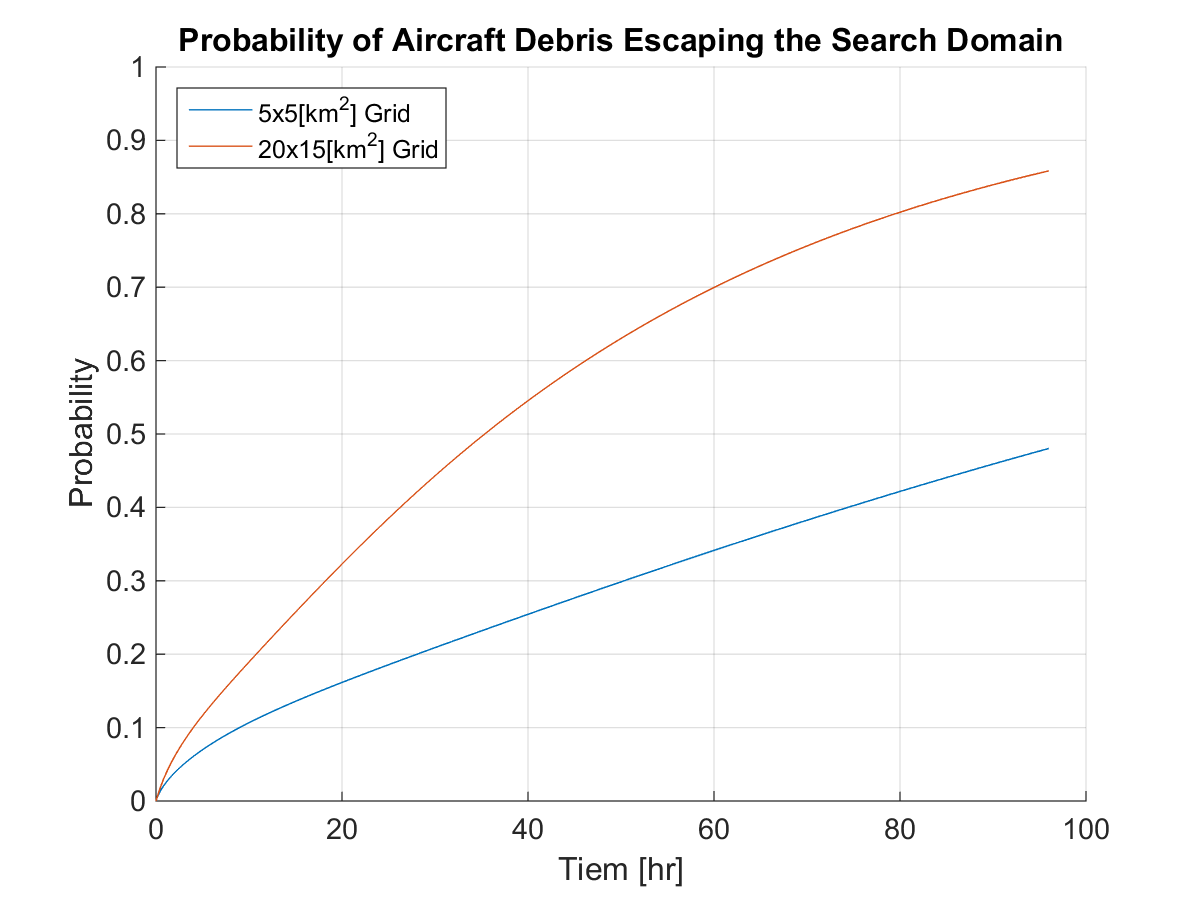
\includegraphics[width=0.8\linewidth]{simulation/NoSearchEscapeExplain}
		\caption{Decrease in grid cell resolution causes higher numerical leakage}
		\label{fig:NoSearchEscapeExplain}
	\end{figure}
\end{center}

In Figure \ref{fig:NoSearchEscapeExplain}, it is evident that reduction in cell resolution causes the Markov drifting simulation leakage.

%\newpage

%%%%%%%%%%%%%%%%%%%%%%%%%%%%%%%%%%%%%%%%%%%%%%%%%%%%%%%%%%%%%%%%%%
\section{Strengths and Weaknesses}\label{sec:sandw}
%%  You can write most of this section before 100\% of your results are done if your coding is running a little behind.  It doesn't have to be exactly 5 bullet points, just whatever makes sense given your paper.


\textit{Strengths:}
\begin{itemize}
\item \textbf{simple}.  Description.
\item \textbf{Requires no input data for the ocean drift}. Saves lots of measurement and preparation time.
\item \textbf{Can be transformed into desired terrain with ease}.  Conformal mapping.
\item \textbf{Short bullet point}.  Description.
\item \textbf{Short bullet point}.  Description.
\end{itemize}
\ \\
\noindent \textit{Weaknesses:}
\begin{itemize}
\item \textbf{Require a fine grid resolution for realistic results}. Excessive discretization can cause unwanted error in total escape probability. See Section \ref{sec:sensitive} and Figure \ref{fig:NoSearchEscapeExplain}.
\item \textbf{}.  Description.
\item \textbf{very simplified drift modeling}.  Description.
\item \textbf{Short bullet point}.  Description.
\item \textbf{Short bullet point}.  Description.
\end{itemize}






%%Uncomment below if you want to begin the next section on a newpage:
%\newpage

%%%%%%%%%%%%%%%%%%%%%%%%%%%%%%%%%%%%%%%%%%%%%%%%%%%%%%%%%%%%%%%%%%

\section{Conclusion}\label{sec:conclusion}

%%  Almost there!  Time to highlight your most important policy recommendations based on the data you observed.

%% A couple paragraphs summarizing everything, then big bullet points to finish:

\begin{itemize}
\item \textbf{Recommendation 1}.  Why the data says so.
\item \textbf{Recommendation 2}.  Why the data says so.
\item \textbf{Recommendation 3}.  Why the data says so.
\item \textbf{Recommendation 4}.  Why the data says so.
% Exact Number of recommendations isn't important
\item \textbf{Make Sure to form a team of search agents that would not give up the search half way}.  One person contributing is $\lll$ two person $\lll$ three person, etc.
\end{itemize}




%%Uncomment below if you want to begin the next section on a newpage:
%\newpage

%%%%%%%%%%%%%%%%%%%%%%%%%%%%%%%%%%%%%%%%%%%%%%%%%%%%%%%%%%%%%%%%%%

%%%This is your bibliography.  Build it up as you go.

\begin{thebibliography}{99}
%%  The {99} can be any number that is at least as big as the number of articles you are citing.  You can leave it at 99.


%% Here's how to do a bibliography entry.  The exact citation format doesn't matter too much.  Change it if you like.


%\bibitem{NameofItem1}  Author, Initial.  ``Title."  \emph{Journal} \textbf{Volume} (Year) pagestart--pageend.

\bibitem{10uscg} Kratzke, T.M.; Stone, L.D.; Frost, J.R. ``Search and Rescue Optimal Planning System" \emph{Information Fusion (FUSION), 2010 13th Conference on} \textbf{DOI:10.1109/ICIF.2010.5712114} 
(2010) 1-8 

\bibitem{83stone}  Stone, L. D.  ``The Process of Search Planning: Current Approaches and Continuing Problems."  \emph{Operations Research} \textbf{31(2)} (1983): 207-233.

\bibitem{46koopman}  Koopman, B.O.  ``Search and Screening."  \emph{Operation Evaluation Research Group Report} \textbf{56} (1946) Center for Naval Analysis; See also: ``The Theory of Search, I-III" \emph{Operations Research} (1956) \textbf{4} 324-246; (1956) \textbf{4} 503-531;  (1957) \textbf{5} 613-626. 

\bibitem{13kagan}  Kagan, E.;Ben-Gal, I.  ``Probabilistic Search for Tracking Targets: Theory and Modern Applications."  \emph{WILEY} (2013) 19-313.

%\bibitem{NameofItem2}  NameofOnlineResourceorGovernmentAgency. ``Title.'' \url{http://www2.census.gov/census_2000/datasets/Summary_File_1/New_York/}

\bibitem{uav} 

\bibitem{heli} U.S. Coast Guard Acquisition Directorate. ``Aviation Fact Sheet." \url{http://www.uscg.mil/acquisITION/programs/pdf/air.pdf}

\bibitem{vessel} Damen Shipyards, ``NH 1816: a New Type of Search and Rescue boat for KNRM" \emph{Maritime by Holland} (2014) \textbf{63} 41-43
\url{http://products.damen.com/~/media/Products/Images/Clusters\%20groups/High\%20Speed\%20Crafts/Search\%20and\%20Rescue\%20Vessel\%201906/Documents/Maritime_by_Holland_2014_Magazine.ashx}

\end{thebibliography}

% Now you can automatically cite your articles by typing \cite{NameofItem1} in your paper.



%%%%%%%%%%%%%%%%%%%%%%%%%%%%%%%%%%%%%%%%%%%%%%%%%%%%%%%%%%%%%%




%%%Optional appendix suggestions:  (or you can print these out separately)
\newpage
\appendix
\appendixpage
\addappheadtotoc \setcounter{page}{1} \rhead{Appendix Page \thepage\
of \pageref{LastPage}}
\subsection*{Appendix A: Computer Code}
\singlespacing
\paragraph{main.m}:
\lstinputlisting{./simulation/main.m}
\subsection*{Appendix B: Full-Page Plots}


\end{document}


% Hope this was helpful.  Let me know if you win!  --spann